\section[King Harald's Wedding]{
    
\includegraphics[width=9.3cm]{viking-tales/030}\\
    King Harald's Wedding}

\lettrine{I}{t} had taken King Harald ten years to fight so many battles.
And all that time he had not cut his hair or combed it. Now he was
feasting one day at an earl's house. Many people were there.

``How is it, friends?'' Harald said. ``Have I kept my vow?''

His friends answered:

``You have kept your vow. There is no king but you in all Norway.''

``Then I think I will cut my hair,'' the king laughed.

So he went and bathed and put on fresh clothes. Then the earl cut his
hair and beard and combed them and put a gold band about his head. Then
he looked at him and said:

``It is beautiful, smooth, and yellow.''

And all people wondered at the beauty of the king's hair.

``I will give you a new name,'' the earl said. ``You shall no longer be
called Shockhead. You shall be called Harald Hairfair.''

``It is a good name,'' everybody cried.

Then Harald said:

``But I have another thing to do now. Guthorm, you shall take the same
message to Gyda that you gave ten years ago.''

So Guthorm went and brought back this answer from Gyda:

``I will marry the king of all Norway.''

So when the wedding time came, Harald rode across the country to the
home of Gyda's father, Eric. Many men followed him. They were all richly
dressed in velvet and gold.

For three nights they feasted at Eric's house. On the next night Gyda
sat on the cross-bench with her women. A long veil of white linen
covered her face and head and hung down to the ground. After the
mead-horns had been brought in, Eric stood up from his high seat and
went down and stood before King Harald.

``Will you marry Gyda now?'' he asked.

\begin{figure}
    \centering
    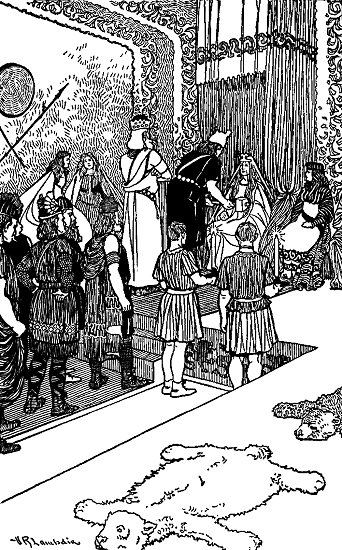
\includegraphics[width=9.1cm]{viking-tales/031}
    \caption{``I, Harald, King of Norway, take you Gyda, for my wife''}
\end{figure}

Harald jumped to his feet and laughed.

``Yes,'' he said. ``I have waited long enough.''

Then he stepped down from his high seat and stood by Eric. They walked
about the hall. Before them walked thralls carrying candles. Behind them
walked many of King Harald's great earls. Three times they walked around
the hall. The third time they stopped before the cross-bench. King
Harald and Eric stepped upon the platform, where the cross-bench was.

Eric gave a holy hammer to Harald, and it was like the hammer of Thor.
Harald put it upon Gyda's lap, saying:

``With this holy hammer of Thor's, I, Harald, King of Norway, take you,
Gyda, for my wife.''

Then he took a bunch of keys and tied it to Gyda's girdle, saying:

``This is the sign that you are mistress of my house.''

After that, Eric called out loudly:

``Now, are Harald, King of Norway, and Gyda, daughter of Eric, man and
wife.''

Then thralls brought meat and drink in golden dishes. They were about to
serve it to Gyda for the bride's feast, but Harald took the dish from
them and said:

``No, I will serve my bride.''

So he knelt and held the platter. When he did that his men shouted. Then
they talked among themselves, saying:

``Surely Harald never knelt before. It is always other people who kneel
to him.''

When the bride had tasted the food and touched the mead-horn to her lips
she stood up and walked from the hall. All her women followed her, but
the men stayed and feasted long.

On the next morning at breakfast Gyda sat by Harald's side. Soon the
king rose and said:

``Father-in-law, our horses stand ready in the yard. Work is waiting for
me at home and on the sea. Lead out the bride.''

So Eric took Gyda by the hand and led her out of the hall. Harald
followed close. When they passed through the door Eric said:

``With this hand I lead my daughter out of my house and give her to you,
Harald, son of Halfdan, to be your wife. May all the gods make you
happy!''

Harald led his bride to the horse and lifted her up and set her behind
his saddle and said:

``Now this Gyda is my wife.''

Then they drank the stirrup-horn and rode off.

``Everything comes to King Harald,'' his men said; ``wife and land and
crown and victory in battle. He is a lucky man.''

\begin{figure}[hb]
    \centering
    \vskip8pt
    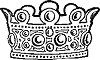
\includegraphics[width=2.7cm]{viking-tales/014}
\end{figure}
